\documentclass[tikz,border=10pt]{standalone}
\begin{document}
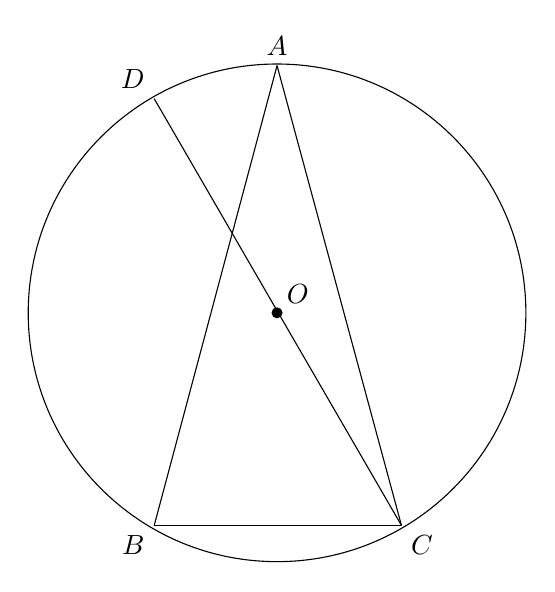
\begin{tikzpicture}
  \coordinate (O) at (0,0);
  \coordinate (A) at (0,3.14);
  \coordinate (B) at (-1.56,-2.70);
  \coordinate (C) at (1.58,-2.70);
  \coordinate (D) at (-1.56,2.72);

  \draw (O) circle (3.16);

  \draw (A) -- (B);
  \draw (A) -- (C);
  \draw (B) -- (C);
  \draw (D) -- (C);

  \fill (O) circle (2pt);

  \node[above] at (A) {$A$};
  \node[above left] at (D) {$D$};
  \node[above right] at (O) {$O$};
  \node[below left] at (B) {$B$};
  \node[below right] at (C) {$C$};
\end{tikzpicture}
\end{document}
